\begin{figure}[htbp]
\centering
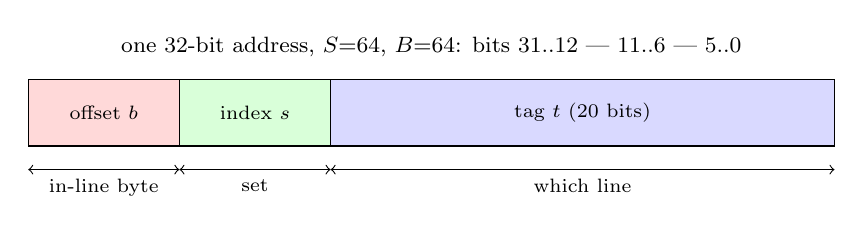
\begin{tikzpicture}[font=\footnotesize, x=3.2mm, y=6mm]
  \draw (0,0) rectangle (32,1.4);
  \draw[fill=red!15]  (0,0) rectangle (6,1.4);
  \draw[fill=green!15](6,0) rectangle (12,1.4);
  \draw[fill=blue!15] (12,0) rectangle (32,1.4);
  \node at (3,0.7) {\scriptsize offset $b$};
  \node at (9,0.7) {\scriptsize index $s$};
  \node at (22,0.7) {\scriptsize tag $t$ (20 bits)};
  \draw[<->] (0,-0.5) -- (6,-0.5) node[midway,below]{\scriptsize in-line byte};
  \draw[<->] (6,-0.5) -- (12,-0.5) node[midway,below]{\scriptsize set};
  \draw[<->] (12,-0.5) -- (32,-0.5) node[midway,below]{\scriptsize which line};
  \node at (16,2.1) {one 32-bit address, $S{=}64$, $B{=}64$: bits 31..12 | 11..6 | 5..0};
\end{tikzpicture}
\caption{The address split for $S{=}64$ sets and $B{=}64$-byte lines:
the low 6 bits are the \texttt{offset} (byte within the line), the next
6 are the set \texttt{index}, and the remaining 20 bits are the
\texttt{tag} that tells lines sharing a set apart. Every cache geometry
question reduces to where these boundaries fall.}
\label{fig:split10}
\end{figure}
